\documentclass{minimal}

\usepackage{tikz}
\usetikzlibrary{calc, arrows, fit, positioning}
\definecolor{clamped}{RGB}{200,200,200}

\begin{document}
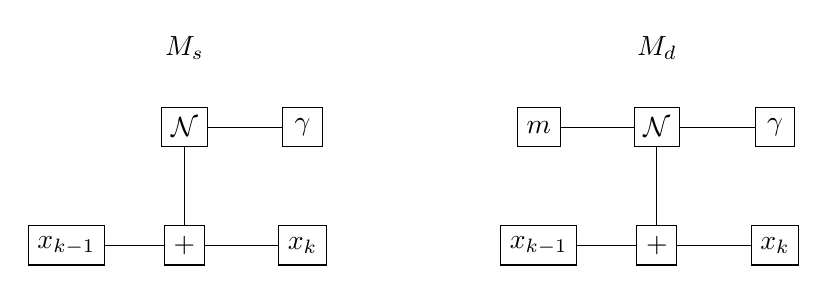
\begin{tikzpicture}
    [
        node distance=15mm,auto,>=latex',
        box/.style={draw, minimum size=.5cm},
        bbox/.style={draw, minimum size=1cm},
        blackbox/.style={draw, fill=black, minimum size=0.25cm}
    ]
    \tikzstyle{line} = [draw, -latex,>=latex]
    \tikzstyle{dash} = [dashed, -latex,>=latex]
    \tikzstyle{branch} = [fill,shape=circle,minimum size=3pt,inner sep=0pt]
    
    \begin{scope}
        \node[box] (add) {+};
        \node[box, left of=add] (x_k_min) {$x_{k-1}$};
        \node[box, right of=add] (x_k) {$x_{k}$};
        \node[box, above of=add] (N) {$\mathcal{N}$};
        \node[box, right of=N] (gam) {$\gamma$};

        \path[line] (add) edge[-] (x_k_min);
        \path[line] (add) edge[-] (x_k);
        \path[line] (add) edge[-] (N);
        \path[line] (N) edge[-] (gam);

        \node[above of=N, node distance=1.0cm] {$M_s$};
    \end{scope}

    \begin{scope}[shift={(6.0cm, 0.0cm)}]
        \node[box] (add) {+};
        \node[box, left of=add] (x_k_min) {$x_{k-1}$};
        \node[box, right of=add] (x_k) {$x_{k}$};
        \node[box, above of=add] (N) {$\mathcal{N}$};
        \node[box, right of=N] (gam) {$\gamma$};
        \node[box, left of=N] (m) {$m$};

        \path[line] (add) edge[-] (x_k_min);
        \path[line] (add) edge[-] (x_k);
        \path[line] (add) edge[-] (N);
        \path[line] (N) edge[-] (gam);
        \path[line] (N) edge[-] (m);

        \node[above of=N, node distance=1.0cm] {$M_d$};
    \end{scope}

\end{tikzpicture}
\end{document}